\section{Auswertung}

\begin{frame}{Inhaltsverzeichnis}
    \tableofcontents[currentsection, hidesubsections]
\end{frame} 

\subsection{Maße}

\begin{frame}[t]{Auswertung}
    \begin{block}{Maße}
    Masse: $m = \SI{435.64}{\gram}$

    Höhe über dem Boden: $l= \SI{26.4}{\centi\meter}$
    
    Radius des Rades: $R =\SI{6.35}{\centi\meter}$
    
    Radius der Drehachse zur Mitte (einfache Messung): $r= \SI{3}{\milli\meter}$
    \end{block}
\end{frame}
\subsection{Berechneter Radius}
\begin{frame}[t]{Auswertung}

    \begin{block}{Berechneter Radius}
        Der Radius ergibt sich zu $r= \SI{3.279}{\milli\meter}$. 
    \end{block}
\end{frame}

\subsection{Plots - lineare Regression}

\begin{frame}{Auswertung}
    \begin{figure}   
    
    \centering
    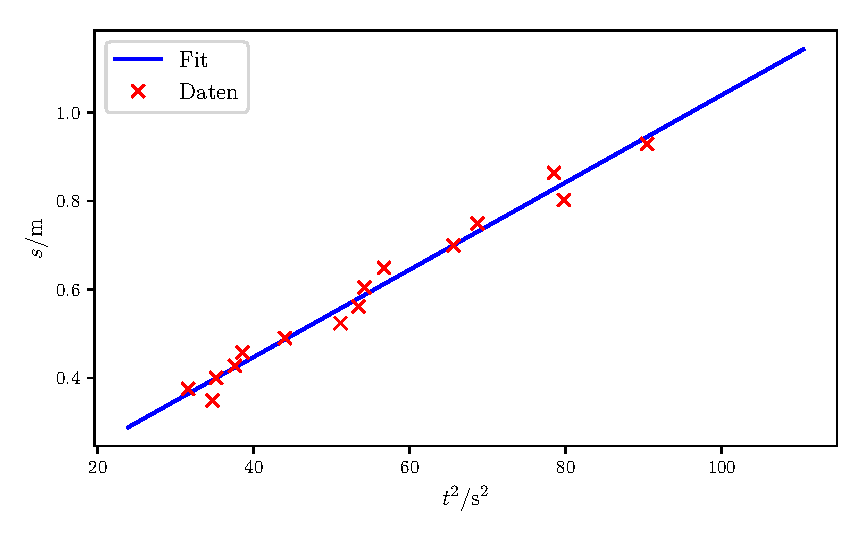
\includegraphics[width=10cm, height=6cm]{build/plot1b.pdf}
    \caption{Die lineare Regression, um die Beschleunigung des Rads zu bestimmen. Dafür wurde die Zeit zum Quadrat gegen die zurückgelegte Strecke aufgetragen. Dies ist die erste Messung.} 

    \label{fig:plot1b}
\end{figure}
\end{frame}

\begin{frame}{Auswertung}
    \begin{figure}   
    
    \centering
    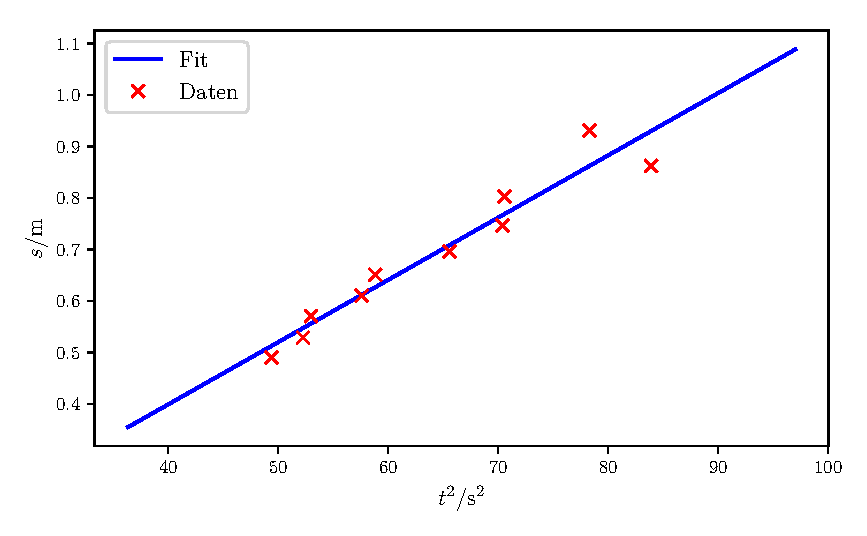
\includegraphics[width=10cm, height=6cm]{build/plot2b.pdf}
    \caption{Die lineare Regression, um die Beschleunigung des Rads zu bestimmen. Dafür wurde die Zeit zum Quadrat gegen die zurückgelegte Strecke aufgetragen. Dies ist die zweite Messung.} 

    \label{fig:plot2b}
\end{figure}
\end{frame}

\begin{frame}{Auswertung}
    \begin{figure}   
    
    \centering
    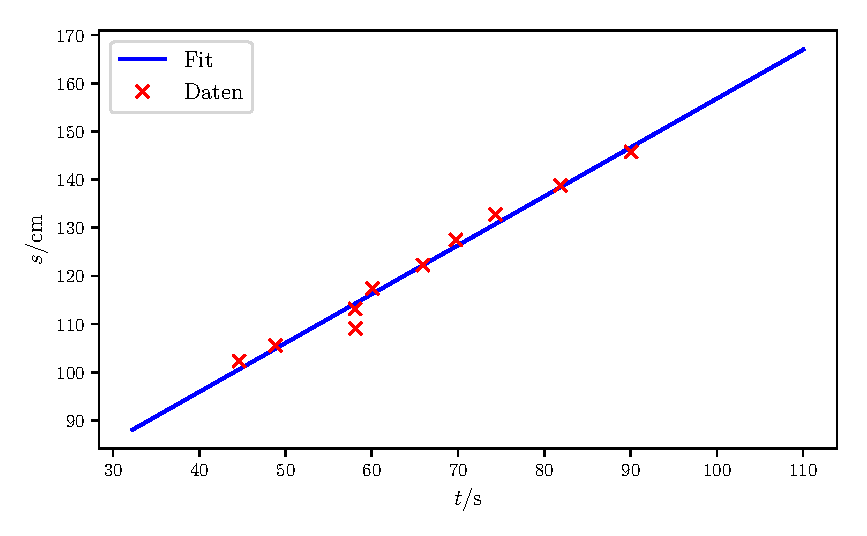
\includegraphics[width=10cm, height=6cm]{build/plot3b.pdf}
    \caption{Die lineare Regression, um die Beschleunigung des Rads zu bestimmen. Dafür wurde die Zeit zum Quadrat gegen die zurückgelegte Strecke aufgetragen. Dies ist die dritte Messung.} 

    \label{fig:plot3b}
\end{figure}
\end{frame}

\subsection{Beschleunigung}
\begin{frame}{Auswertung}
    \begin{block}{Beschleunigung}
        
        Die mittlere Beschleunigung ergibt sich zu $a = \SI{2.14(197)}{\centi\meter\per\second\squared}$.
        \\Der Wert, der sich für die Beschleunigung nach unserer Theorieformel ergibt, liegt bei $a_\text{theo}= \SI{5.20}{\centi\meter\per\second\squared}$.
    \end{block}
\end{frame}
    
\subsection{Plots - Tatsächliche Daten}
\begin{frame}{Auswertung}
    \begin{figure}   
    
    \centering
    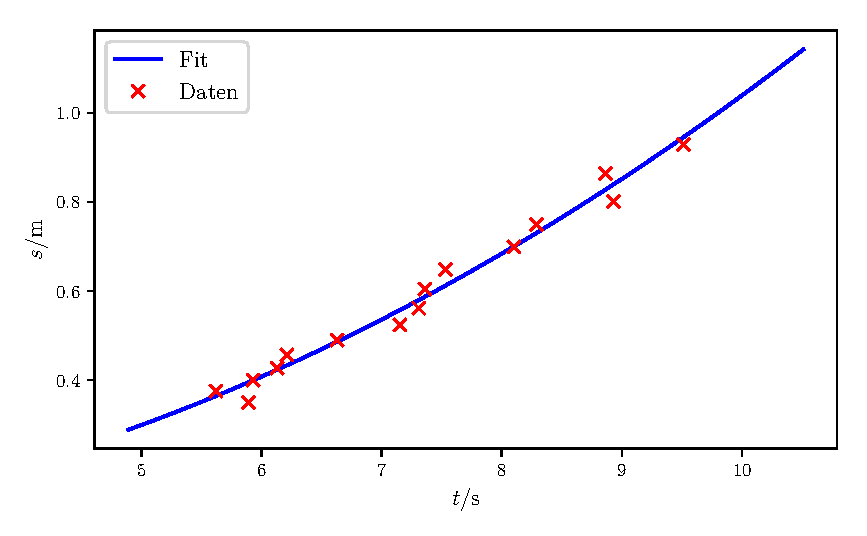
\includegraphics[width=10cm, height=6cm]{build/plot1a.pdf}
    \caption{Hier ist die Strecke gegen die Zeit aufgetragen. Dies ist die erste Messung.} 

    \label{fig:plot1a}
\end{figure}
\end{frame}

\begin{frame}{Auswertung}
    \begin{figure}   
    
    \centering
    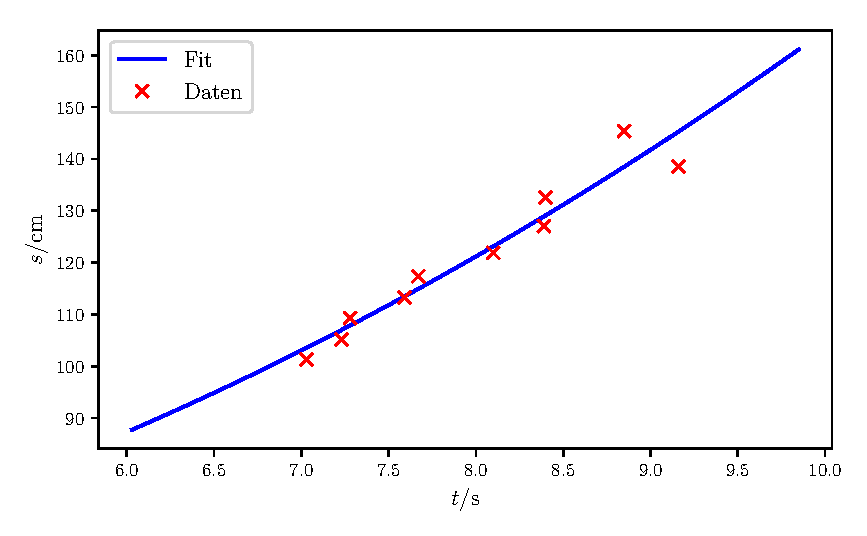
\includegraphics[width=10cm, height=6cm]{build/plot2a.pdf}
    \caption{Hier ist die Strecke gegen die Zeit aufgetragen. Dies ist die zweite Messung.} 

    \label{fig:plot2a}
\end{figure}
\end{frame}

\begin{frame}{Auswertung}
    \begin{figure}   
    
    \centering
    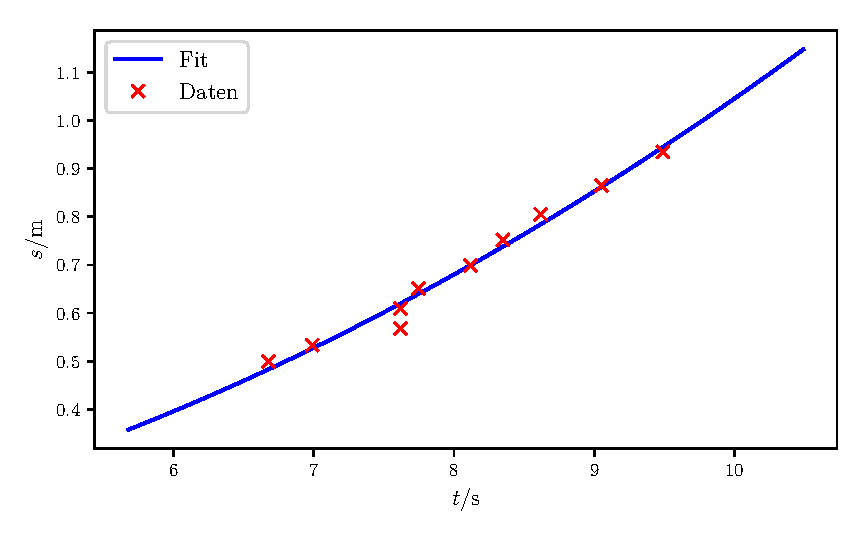
\includegraphics[width=10cm, height=6cm]{build/plot3a.pdf}
    \caption{Hier ist die Strecke gegen die Zeit aufgetragen. Dies ist die dritte Messung.} 

    \label{fig:plot3a}
\end{figure}
\end{frame}
\subsection{Energieerhaltung}
\begin{frame}{Auswertung}
    \begin{figure}   
    
    \centering
    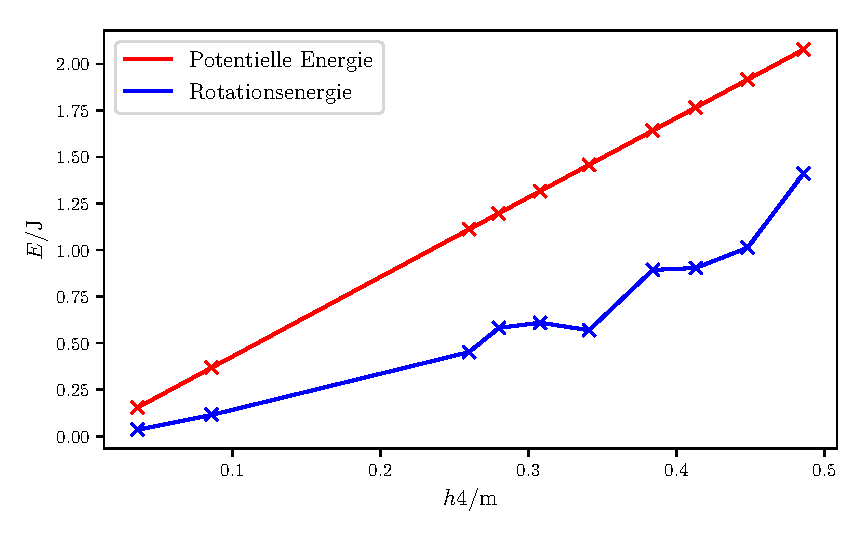
\includegraphics[width=10cm, height=6cm]{build/plot4a.pdf}
    \caption{Die potentielle Energie und die Rotationsenergie gegen die Höhe aufgetragen.} 

    \label{fig:plot4}
\end{figure}
\end{frame}

